% !TEX root = handbook-physics.tex
% !TEX TS-program = pdflatex
% !TEX encoding = UTF-8 Unicode






\chapter[Absorption, Scattering And Dispersion Of Light]{Absorption, Scattering And Dispersion Of Light. Vavilov-Cherenkov Radiation}
\label{ch-34}

\section{Interaction of Light With Matter}
\label{sec-34.1} 


\subsection{}\label{34.1.1} According to the concepts of classical electron theory, the variable electromagnetic field of a light wave, propagating in a dielectric medium, sets up forced vibrations of the bound charges (electrons and ions) included in the composition of the molecules of the -medium. Consequently, each molecule of the medium can be considered as a system of oscillators with different angular frequencies of natural vibration \ssect{28.1.1}. Ions are considerably more massive than electrons and execute appreciable vibration only as the effect of low-frequency (infrared) radiation. In the frequency region of visible and ultraviolet light, the deciding role is played by the forced vibration of the external, more weakly bound electrons of atoms and molecules.
They are called \redem{optical electrons}.

\subsection{}\label{34.1.2} Electrons and ions that execute forced vibrations by the action of light radiate secondary light waves of the same frequency. The average distance between the molecules of a medium is only a small fraction of the coherence length \ssect{32.1.4} of the light. Therefore, the secondary waves radiated by a great number of neighbouring molecules are coherent and display interference when superposed.

If the medium is homogeneous and isotropic \ssect{30.1.6}, interference results in the formation of a transmitted wave, whose phase velocity depends upon the frequency and whose direction of propagation coincides with that of the primary wave.

\subsection{}\label{34.1.3} When the medium is optically nonhomogeneous, the superposition of the primary and secondary waves results in scattering of the light \ssect{34.3.1}. Finally, when light falls on the interface between two different media, interference results in the formation of a reflected wave in addition to the transmitted wave. Thus, a more or less considerable layer of particles of the medium, adjoining the reflecting surface, participates in the formation of the reflected wave. Therefore, upon total internal reflection \ssect{31.5.8}, the electromagnetic field of the light wave is not completely cut off at an interface with an optically less dense medium, but partly penetrates it. The field strength E, however, decreases very rapidly as the distance to the interface increases according to the equation 
\begin{equation*}%
E \propto \exp \left[ -\frac{2\pi z}{\lambda_{2}}\sqrt{ \left(\sin^{2}\dfrac{i}{n_{21}^{2}} \right) - 1 }\right],
\end{equation*}
where $z$ is the distance from the interface, $i$ is the angle of incidence $(i > i_{cr})$, $\lambda_{2}$ is the wavelength of light in the medium, $i_{cr}$ is the critical angle \ssect{31.5.8}, and $n_{21}$ is the relative refractive index of the medium.

\section{Absorption of Light}
\label{sec-34.2} 


\subsection{}\label{34.2.1} The \redem{absorption of light} refers to the reduction in the energy of a light wave as it is propagated in a substance. It results from the conversion of energy of the wave into internal energy \ssect{9.1.2} of the substance or into energy of secondary radiation having a different spectral composition and other directions of propagation (photoluminescence, Section \ssect{39.7.5}. Light
absorption may lead to heating of the substance, excitation and ionization of its atoms or molecules, photochemical reactions and other processes in the substance.

The absorption of light is described by the \redem{Bouguer-Lambert law} (also called the \redem{Lambert law}), which states that the intensity $I$ of a plane wave of monochromatic light decreases as it passes through an absorbing medium according to the exponential relation
\begin{equation*}%
I = I_{0} \exp (-\alpha x),
\end{equation*}
where $I_{0}$ and $I$ are the intensities of the light at the entrance to and exit from a layer of the medium of thickness $x$, and $\alpha$ is the \redem{absorption factor} (\redem{linear coefficient of absorption}), which depends on the chemical nature and state of the substance and on the wavelength $\lambda$ of the light.

\redem{Beer's law} is valid for dilute solutions of an absorbing substance in a nonabsorbing solvent: $\alpha = bc$, where $c$ is the concentration of the solution and $b$ is a proportionality factor that is independent of $c$. Beer’s law does not hold for high concentrations because of the effect of the interaction between the closely spaced molecules of the absorbing substance.

\subsection{}\label{34.2.2} According to the Bouguer-Lambert law, the equation of a plane, linearly polarized, monochromatic light wave, propagating in an absorbing medium along the positive direction of the $OX$ axis, is of the form:
\begin{equation*}%
E = E_{0}\exp \left( - \frac{\alpha x}{2} \right) \cos ( \omega t- kx).
\end{equation*}
Here $E$ is the strength of the wave’s electric field at points with the coordinate $x$, $E_{0}$ is the amplitude of $E$ at points in the plane $x = 0$, $\omega$ is the angular frequency of the light, $k = 2 \pi/\lambda = \omega n/c$ is the wavenumber, $\lambda$ is the wavelength of the light in
the medium, $c$ is the velocity of light in free space, and $n$ is the refractive index of the medium.

In the exponential form the equation of this wave is of the form \ssect{30.2.7}:
\begin{equation*}%
E = E_{0}\exp \left( - \frac{\alpha x}{2} \right) \exp i \left( \omega t- kx \right) = E_{0} \exp i \left( \omega t- \dfrac{\tilde{n} \omega x}{c}  \right)
\end{equation*}
where 
\begin{equation*}%
\tilde{n} = n \left(1 - i \frac{\alpha \lambda}{4 \pi}\right) = (1 - i\varkappa),
\end{equation*}
is the \redem{complex refractive index of the medium} $(i = \sqrt{-1})$, and $\varkappa = \alpha/2k = \alpha \lambda/4\pi$ is the \redem{absorptivity}, or \redem{absorptive power}, which characterizes the decrease in the intensity and amplitude of a plane wave as it propagates in a medium.

\subsection{}\label{34.2.3} The dependence of the absorption factor $\alpha$ of a dielectric on the light’s wavelength $\lambda$, characterizing the \redem{light absorption spectrum} in this medium, is related to the resonance phenomenon
upon forced vibration of the electrons in the atoms and the
atoms in the molecules of the dielectric. Dielectrics absorb light more or less selectively: absorption is great only in frequency regions close to the natural frequencies of vibrations of the electrons in the atoms and the atoms in the molecules. This phenomenon of \redem{resonance absorption of light} is displayed most clearly in dilute monatomic gases (for example, the vapours of most metals), which have a \redem{line spectrum of light absorption}. Discrete frequencies of intensive light absorption coincide with
the frequencies of the self-radiation of excited atoms in these gases.

Systems of closely spaced lines, forming \redem{absorption bands}, are observed in gases having polyatomic molecules. The structure of the absorption bands is determined by the composition and structure of the molecules. Liquid and solid dielectrics have \redem{continuous absorption spectra}, consisting of comparatively wide absorption bands, within which the absorption factor $\alpha$ reaches a quite high value and varies smoothly in accordance with the wavelength $\lambda$. This kind of dependence of $\alpha$ on $\lambda$ in condensed media is due to the strong interaction between the particles of the medium, leading to the appearanceof a great number of additional resonance frequencies.

\subsection{}\label{34.2.4} At sufficiently high intensities of light, deviations from the Bouguer-Lambert law \ssect{34.2.1} are observed: the absorption factor of a dielectric medium begins to depend upon $I$, decreasing with an increase in $I$. This phenomenon, inexplicable within the framework of classical light absorption theory, is readily interpreted in the quantum theory of the interaction of light with matter. In the absorption of light, a part of the molecules of the medium goes over into an excited state. The excited molecules
cannot participate in further light absorption until they
return, after expending their surplus energy, to the unexcited
(“normal”) state. The higher the intensity of the light and the longer the average lifetime $\expval{\tau}$ of a molecule in the excited state, the greater the fraction of excited molecules in the medium. 

If this fraction of excited molecules is negligible, light is absorbed in accordance with the Bouguer-Lambert law. Otherwise, $\alpha$ decreases with an increase in the intensity of the light. It is feasible to obtain a nonequilibrium state of the medium, in which the fraction of excited molecules is so large that the absorption factor of the medium becomes negative. This phenomenon is made use of in a quantum oscillator of radio waves and light \ssect{39.8.8}.

\subsection{}\label{34.2.5} Metals in a condensed state contain a huge amount of conduction electrons and, therefore, have high electrical conductance. When subjected to light, the conduction electrons execute variable motion and radiate secondary waves. As a result of the superposition of the primary wave, falling on the surface of the metal, and the secondary wave, an intensive reflected wave is formed and a relatively weak wave that enters the metal. The reflection coefficient \ssect{31.5.6} can reach 95 per cent and even more. It depends upon the surface finish of the metal, its electrical conductance and the light frequency. 

The refracted wave is rapidly absorbed in the metal. Its energy is consumed on the production of Joule heat, evolved by the conduction currents initiated by the action of light in the thin layer of metal adjacent to the surface. In the  frequency region of infrared radiation, the optical properties of metals are determined mainly by the conduction electrons. But in the region of visible light and especially ultraviolet radiation, bound electrons, in the ions of the metal, begin to play an appreciable role. This leads to a reduction in the reflection coefficient and to its pronounced dependence on the frequency.

\section{Scattering of Light}
\label{sec-34.3} 


\subsection{}\label{34.3.1} The \redem{scattering of light} is the phenomenon in which light is transformed by a substance. It is accompanied by a change in the direction of light propagation, and is manifested as an extrinsic glow of the substance. This glow is due to the forced vibration of the electrons in the atoms of the scattering medium by the action of the incident light. Light scattering occurs in an optically nonhomogeneous medium, whose refractive index varies irregularly from point to point due either to fluctuations
in the density of the medium or to the presence in it of small
foreign particles. In the former case, \redem{the light scattering} is said to be \redem{molecular} or \redem{Rayleigh scattering}; in the second, \redem{light scattering in a turbid medium}. Examples of turbid media are aerosols (smoke and fog), emulsions and colloidal solutions.

\subsection{}\label{34.3.2} The scattering of light in turbid media by particles whose size is small compared to the wavelength $\lambda$, is called the \redem{Tyndal effect}. A system of electrons, executing forced vibration in the
atoms of electrically isotropic particles of small size $r_{0} \approx $ (0.1 to 0.2) $\lambda$, is equivalent to one oscillating electrical dipole (linear harmonic oscillator). This dipole oscillates at the frequency $\nu$ of the light incident on it, and the intensity of the light it
radiates is proportional to $\nu^{4}$ \ssect{31.3.3}. Hence, \redem{the Rayleigh law} is valid for scattered light. It states that the intensity $I$ of scattered light is inversely proportional to the fourth power of the wavelength: $I \propto \lambda^{-4}$. When white light passes through a finely
divided turbid medium, short-wave (dark-to-light blue) light
predominates in the scattered light, and long-wave (yellow-to-
red) light in the transmitted light. This explains, for instance, the light-blue colour of the sky and the yellowish-red colour of the rising and setting sun.

In scattering of natural light \ssect{34.1.1}, the dependence of the intensity of the scattered light on the scattering angle $\theta$ is of the form:
\begin{equation*}%
I_{\theta} = I_{\pi/2} \, (1 + \cos^{2} \theta).
\end{equation*}
Here $I_{\theta}$ and $I_{\pi/2}$ are the intensities of light scattered at angles of $\theta$ and $\pi/2$ to the direction of the primary light beam falling on a turbid medium. Light scattered at the arbitrary angle $\theta$ is partly polarized \ssect{35.1.1}; that scattered at the angle $\pi/2$ is
completely linearly polarized \ssect{31.1.7}: vector $\vb{E}$ of the field set up by this light is perpendicular to the plane passing through the incident and scattered rays.

\subsection{}\label{34.3.3} As the size $r_{0}$ of the inhomogeneities in a turbid medium is increased, the laws of light scattering are changed. At $r_{0} > \lambda$,
the dependence of $I_{\theta}$ on $\theta$ is of complex form, the intensity of the forward scattering of light (in the directions $\theta < \pi/2$) being greater than for backward scattering. This phenomenon is called the \redem{Mie effect}. In this case, light scattered at the angle $\theta = \pi/2$ is only partly polarized. The dependence of the scattered light intensity $I$ on the wavelength $\lambda$ is of the form: $I \propto \lambda^{-p}$, where $p < 4$ and decreases with an increase in $r_{0}$. At $r_{0} > \lambda$, the spectral compositions of the scattered and incident light practically coincide. This explains, for instance, the white colour
of the clouds.

\subsection{}\label{34.3.4} Molecular scattering in pure media, not containing any foreign impurities, is due to inhomogeneitics that occur in the process of random thermal motion of the particles of the medium. These inhomogeneities are associated with fluctuations in density \ssect{11.6.1}, whereas in media having anisotropic (polar) molecules,
the inhomogeneities are also due to fluctuations in the
orientation of these molecules (fluctuations of anisotropy). In
true solutions, light may be scattered by fluctuations in concentration.

Under ordinary conditions the size of the regions of the
medium, corresponding to any appreciable fluctuations, is much
less than the wavelength of visible light. Therefore, the dependence of the scattered light intensity on the wavelength $\lambda$ and angle $\theta$, as well as on the kind of polarization in molecular scattering, is analogous to the corresponding laws for the Tyndal effect. But, in contrast to the Tyndal effect, the intensity of molecular scattering of light depends upon the temperature of the medium, increasing with the temperature.

\section{Normal and Anomalous Light Dispersion}
\label{sec-34.4} 



\subsection{}\label{34.4.1} The \redem{dispersion of light} is the dependence of its phase velocity $v$ in a medium on its frequency $\nu$. According to Section \ssect{31.5.1}, $v = c/n$, where $c$ is the velocity of light in free space, and $n$ is the refractive index of the medium. Since $c$ is a universal constant, the same for electromagnetic waves of any frequency, the existence of the dispersion of light in a medium is due to the fact that' its refractive index n depends upon the frequency $\nu$. This dependence is readily detected, for example, in pas­sing a beam of white light through a prism made of some transparent medium. Observed on the screen, mounted behind the prism, is an iridescent band (\figr{fig-34-01}) called a \redem{prismatic}, or \redem{dispersion spectrum}.

\begin{figure}%[-3cm]
\centering
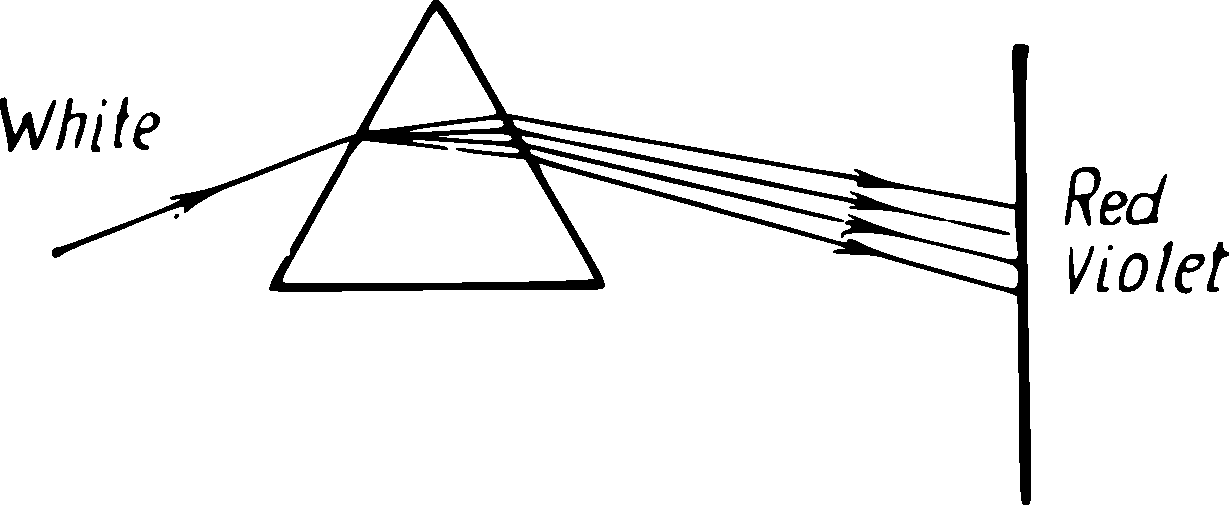
\includegraphics[width=0.8\textwidth]{figs/ch-34/fig-34-01.pdf}
\sidecaption{Prismatic dispersion of light.\label{fig-34-01}}
\end{figure}

\subsection{}\label{34.4.2} The dependence of the refractive index $n$ of a medium on the light frequency $\nu$ is neither  linear nor monotonic. The region of $\nu$ values in which $\dv*{n}{\nu} > 0$, i.e. $n$ increases with $\nu$, corresponds
to \redem{normal dispersion of light}. Normal dispersion is found for substances transparent to light. For example, ordinary glass is transparent to visible light and, in this frequency region, normal dispersion of light is observed in glass. A case of normal dispersion of light is illustrated in \figr{fig-34-01}.

The dispersion of light is said to be \redem{anomalous} if $\dv*{n}{\nu} < 0$, i.e. the refractive index of the medium decreases with an increase in $\nu$. Anomalous dispersion is found in frequency regions that correspond to intensive absorption of light in the given medium \ssect{34.2.1}. In ordinary glass, for instance, these bands are in the infrared and ultraviolet parts of the spectrum.

\subsection{}\label{34.4.3} Depending upon the kind of dispersion light undergoes, its group velocity $u$ can be either more or less than its phase velocity $v$. According to Sect. \ssect{30.4.3}, the group velocity is related to the angular velocity $\omega$ of the wave and to its wave-number $k$ by the equation: $u = \dv*{\omega}{k}$. Since $\omega = 2\pi \nu$ and $k = 2\pi/\lambda = 2\pi n \nu/c$,
\begin{equation*}%
u = \frac{c}{n + \nu \dfrac{\dd n}{\dd \nu}} =  \frac{v}{1 + \dfrac{\nu}{n} \dfrac{\dd n}{\dd \nu}}. 
\end{equation*}
In normal dispersion the group velocity is less than the phase
velocity $(u < v)$. In the case of anomalous dispersion $u > v$ and, in particular, if $n + \nu \dv*{n}{\nu} < 1$, then $u > c$. This does not contradict the statement of the special theory of relativity that the velocity of any signal (including a light signal) cannot exceed $c$ \ssect{5.1.3}. 

The concept of group velocity correctly describes only a signal whose “shape”, i.e. the distribution of amplitudes
and energies along its “length”, does not change when the
signal travels through the medium. But for light, this condition is complied with only approximately; the narrower the frequency spectrum of the signal and the less the light dispersion in the medium, the more exactly the condition is complied with. In the frequency regions corresponding to anomalous dispersion, the group velocity does not coincide with the velocity of the signal because, owing to considerable dispersion of light, the “snape” of the signal changes rapidly as it propagates in the medium.


\section{Classical Electron Theory of Light Dispersion}
\label{sec-34.5} 


\subsection{}\label{34.5.1} Optically transparent media are nonmagnetic (p,r  1),
so that their refractive index \ssect{31.5.1} n = Y £r = Y  + Xe>
where er and %e are the relative permittivity (dielectric constant)
and the dielectric (or electric) susceptibility of the medium
\ssect{18.2.4}. Therefore, the dispersion of light can he regarded
as the dependence of er and Xe on the frequency of the variable electromagnetic field of the light, causing electronic polarization
of the medium \ssect{18.2.2}. If each atom (or molecule) of the
medium contains one optical electron \ssect{34.1.1}, the polarization
vector of the medium \ssect{18.2.3} Pe = -en0 r, where -e is the
charge of the electron, r is its displacement from the equilibrium
position, and n0 is the concentration of atoms (or molecules)
of the medium. On the other hand \ssect{18.2.4}, Pe = e0xeE, where
e0 is the electric constant \ssect{14.2.7}, and E is the strength of the
electric field of the light.

\subsection{}\label{34.5.2} An optical electron executes forced vibrations under the
effect of the following forces:
(a) restoring quasi-elastic force \ssect{40.3.5} Frest = - racogr, where
m and co0 are the mass of the electron and the angular frequency
of its free "undamped vibrations;
(b) force of resistance Fresi = -2Pm dr/dt, where P is the damping
factor of free vibrations of the electron; (c) driving forc F = -eE, exerted on the electron by a variable
field of strength E.
The equation of forced vibrations is
2P- +«gr=
eF
m
In the case of linearly polarized monochromatic light with the
angular frequency co, the field strength E = E0 cos co£, where
E0 = const is the amplitude vector. If, in addition, the medium
does not absorb light, then p = 0 and the steady-state forced
vibration of the optical electron is executed according to the
relation
r =
eE
m (cog-co2)[34
Here the polarization vector of the medium is
rc0e2E  nog2
e m (cog - to2) * e e 0to (wjj - co2) '
The dependence of the refractive index of the medium on co is
of the form
7i2 = l ftp*2
e0m (co- co2)

\subsection{}\label{34.5.3} At values of co close to co0, the absorption of light in the
medium can no longer be neglected, assuming that P = 0. In an absorbing medium (i.e. at P  0), vibrations of the optical
electron and of vector Pe are out of phase with respect to the
oscillations of the field strength E \ssect{29.2.2}:
r = A cos (co£ + <Po)»
where
and tan cp0 = - 2pco
m V ()„2-q)2)2 + 4P*<o*
Accordingly
p = »0g2E0 cos (co t + cpo)
m (cog-co2)2-I- 4P2co2
Introduced to describe the properties of a light-absorbing medium,
along with the complex refractive index \ssect{34.2.2} n =
= n (1 - ix), are the complex dielectric susceptibility %e and the
complex dielectric constant er:
Pe
Xe = and er = l + Xe> whereas n2 = 1 + Xe*
Here Pe and E are complex values of the polarization and
strength of the field:
~ n pF e*(©< + To)  . ,
Pe=---0 0 - -- and E = E 0ew>t.
m /((o§-w2)2 + 4P2co2
so that
ft2 = /12 (1 - iK)2 = l
e*<Po.
8Qm V (o)q - co2)2 + 4p2cc
nQe2 cos cp0
n2 (1 -x*) = l-f
80m Y (a)o - (02)2 + 4p2(02
n0e2 (cog - co2) 
= 1
80m [(cog-co2)2 + 4P2co2] ’
n0e1 sin cp0 2 rc0e2pco
2n2x =
80m Y (co2-co2)2 + 4p2co2 ' 'e0™ [(©§ - co2)2 + 4P2to2] *

\subsection{}\label{34.5.4} In the classical electron theory of light dispersion in
gases, each molecule of the gas is dealt with as a system of q
linear oscillators. If coOJ* and are the natural angular frequency
and damping factor of the ;th oscillator, then
n2 (1 - x2) = 1
Q
nQe2 y
8 0m
3= 1 (ao'i -<o*)« + 4p;ffl*
and
n o.K = noe y
zEl

e0m  (0)- (o2)2+4P*w* *
The dimensionless coefficient fj characterizes the contribution of
the /th oscillator to the dispersion and absorption of light. It is called the oscillator strength. In the classical theory of dispersion,
the values of co07 and fj are assumed to he known from
experimental investigations.
For gases, 1 and n differs only slightly from unity, so that
h2 - 1 = (n + 1) (n - 1) « 2 (n - 1). Therefore, the dependence
of n on co is of the form
+ 280m A ((D2J (B2)2 + 4p2<n2 •
The curve of this equation is shown in Fig. 34.2.
Anomalous dispersion is observed close to each of the frequencies
co07.

\section{Vavilov-Cherenkov Radiation}
\label{sec-34.6} 


\subsection{}\label{34.6.1} Vavilov-Cherenkov radiation (or effect) is the radiation of
light, differing from luminescence \ssect{39.7.1}, emitted in the motion
of charged particles in a substance at velocities V greater
than the phase velocity v of light in this substance. The condition
for the existence of this radiation is: cln < V < c, where c
is the velocity of light in free space (or in vacuum), and n > 1
is the refractive index of the substance.

In the process of Vavilov-Cherenkov radiation, the energy and
velocity of the free emitting particle is reduced, i.e. the particle
Is retarded. But, in contrast to braking radiation (bremsstrah-
i ung) of slowly moving charged particles \ssect{31.3.4}, resulting from
their change in velocity, the reduction in the velocity of particles
in Vavilov-Cherenkov radiation is itself a consequence of this
radiation. In other words, if the loss of energy of the particle,
consumed in emitting Vavilov-Cherenkov radiation, could be
replenished in some way and the particle would continue travelling
in the substance at a “faster-than-light” velocity (V > v),
Vavilov-Cherenkov radiation would still be observed, whereas
there would be no braking radiation in this case.

\subsection{}\label{34.6.2} A charged particle gives rise to short-duration polarization
\ssect{18.2.2} of the substance in the vicinity of the points
through which it travels. Hence, the molecules of the medium,
lying on the path of the particle, become temporarily acting
coherent sources \ssect{30.5.1} of elementary electromagnetic waves
that interfere upon superposition.
If V < v = c/n, the elementary waves cancel one another.
Assuming that the charged particle travels at the velocity V
(where V < v) along the OX axis (Fig. 34.3) and is at points
A and B at the instants of time t and t + A/, respectively. The
distance between A and B is I = VAt. The path difference of
elementary waves, radiated from points A and B in the arbitrary
direction n, making the angle a with vector V, is
It is possible, for each value of the wavelength X, to find a value
I = ia<K at which A = X/2, so that the elementary waves cancel
one another. Thus
l(z% -
When I = radiation, in the direction n from any point M
of portion AB of the path of the charged particle, is cancelled
upon interference with radiation in the same direction from
a like point N on the adjacent portion BC = AB = la, the
distance between points M and N being MN = la Therefore,
upon motion of a charged particle at uniform velocity in a
straight line in a substance at a “slower-than-light” velocity,
the particle docs not emit radiation.

\subsection{}\label{34.6.3} If a particle travels in a substance at a “faster-than-
light” velocity V > v dri, the value of laX, complying with
the condition for the cancelling of elementary waves,
X
laX -
2 v
- - cos a
can be found for all values of angle a, with the exception of
a r c
0 = arc cos - - arc cos -77 - . V nV
For the direction 0 = a, the path difference of the elementary
waves emitted by any two points A and B of the path of the
charged particle (Fig. 34.3) equals zero. Thus
A = DF = (v - V cos 0) At = 0.
Consequently, elementary waves, propagating in the direction
a = 0, reinforce one another upon interference, forming a resultant
radiation in this direction. This is Vavilov-Cherenkov
radiation. Light, emitted at each small portion of the path of
a charged particle, is propagated along the elements of a cone,
whose vertex 0 (Fig. 34.4) is located on this portion and whose35.i] P o l a r i z a t i o n o p L iG H t 4§5
axis coincides with the path of the particle. The elements make
the angle 0 = arc cos (c/nV) with the axis. The light is polarized
so that vector E is normal to the surface of the cone, and
vector II is tangent to it.